\documentclass[a4paper,12pt]{article}
%\documentclass[a4paper,10pt]{scrartcl}

\usepackage{amsmath,amssymb}
\usepackage{epic}
\usepackage{eepic}
\usepackage{bm}
\usepackage{array}
\usepackage{float}
\usepackage{multirow}
\usepackage{fancyhdr}

\usepackage{vmargin}            % red�finir les marges
\usepackage{amsthm}
\usepackage{graphicx,color}


\setmarginsrb{2cm}{0.5cm}{2cm}{1cm}{0cm}{1cm}{0cm}{1cm}
\newtheorem{remark}{Remark}

\newcommand{\normL}[1]{%
\ensuremath{||#1||_{L^2}}}
\newcommand{\normLL}[1]{%
\ensuremath{||#1||_{L^1}}}

\newcommand{\abs}[1]{%
\ensuremath{|#1|}}


\newcommand{\norme}[2]{%
\ensuremath{||#1||_{#2}}}

\renewcommand{\d}[0]{%
\ensuremath{\text{d}}}


\newcommand{\systeme}[1]{%
\ensuremath{\begin{numcases} \quad #1 \end{numcases}}}


\newcommand{\integ}[3]{%
\ensuremath{\displaystyle{\int^{#2}_{#1} #3}}}

\newcommand{\somme}[3]{%
\ensuremath{\displaystyle{\sum^{#2}_{#1} #3 }}}

\newlength{\intwidth}
\DeclareRobustCommand{\fpint}[2]
   {\mathop{%
      \text{%
        \settowidth{\intwidth}{$\int$}%
        \makebox[0pt][l]{\makebox[\intwidth]{$-$}}%
        $\int_{#1}^{#2}$}}}


\title{Potential Flow Around a Regular Body in 2D}
\author{}
\date{}

\begin{document}
\maketitle
\section{Setting of the Problem}

Suppose the fluid flow is described by velocity vector field $u$. The velocity field can be written as the gradient 
of a velocity potential $\phi$. 
\begin{equation}\label{Pr0}
 u=\nabla \phi
\end{equation}

Let us assume that the vector field $u$ is irrotational. It means 
$curl(u)=0$. We can also write
$\nabla\times u=0$.

We consider the flow to be incompressible, we have $\nabla\cdot u=0$. If we substitute ~\eqref{Pr0}, we have
\begin{align}
&\nabla \cdot u=0 \\
 &\nabla \cdot \nabla\phi=0 \\
 &\Delta \phi=0
\end{align}
From here we get:
\begin{equation} \label{Pr1}
 \Delta \phi=0
\end{equation}

Let us consider a fluid in an infinite domain. Far from the obstacle, we suppose that the velocity is uniform. Without loss of generality, 
we assume that its direction is $\vec{e_x}$. 
This condition can be written as
\begin{equation} \label{Pr2}
u=u_0\vec{e_x} \quad \text{as }|x|\to\infty, |y|\to\infty
\end{equation}
From ~\eqref{Pr1} and ~\eqref{Pr2}, we obtain the system:
\begin{align} \label{problem1}
\Delta \phi &=0\\
u=\nabla \phi &\to u_0 \vec{e_x} \quad \text{as } x\to\pm\infty
\end{align}
Without any abstacle, this problem has the obvious solution i.e $\phi= u_0 x$.

Let us add a regular obstacle $\Omega_0$. We consider $\partial\Omega_0$ to be $C^1$. It means the obstacle doesn't have any angles nor discontinuities. 
On the border of the obstacle, the velocity is tangential.
\begin{equation}\label{eq1}
u\cdot n=0
\end{equation}
with $n$ is the (exterior) normal vector of $\Omega_0$.
We substitute $u=\nabla\phi$ to~\eqref{eq1}, we get 
\begin{equation}\label{Pr3}
\nabla\phi\cdot n=0
\end{equation}
Equation~\eqref{Pr3} is called an homogeneous Neumann boundary condition.  

From equation~\eqref{Pr0},~\eqref{Pr1},~\eqref{Pr2} and~\eqref{Pr3}, we obtain the problem:
\begin{align} \label{problem2}
\Delta \phi=0 \quad \text{On: } \mathbb{R}^2 \setminus \overline{\Omega_0}=\Omega\\
u=\nabla\phi\to u_0\vec{e_x}\quad \text{as } x \to \pm\infty\\
\nabla\phi \cdot n=0 \quad \partial \Omega_0=\Gamma_0
\end{align}
The problem is hence to find the harmonic function that satisfies all the boundary conditions.

Without the obstacle, problem~\eqref{problem1} has solution $u_0x$. We can use it to find $\phi$. Let us perform a change of variable in order to get the solution of problem~\eqref{problem2}.
Let us define 
\begin{equation}
\psi=\phi-u_0 x \label{changevar} 
\end{equation}
If we substitute~\eqref{changevar} to the problem~\eqref{problem2} we can obtainas follows:
\begin{align}
 \Delta \psi &= \Delta \phi-\Delta (u_0x)\\
\Delta \psi &= \Delta \phi\\
\nabla \psi &= \nabla\phi-u_0\vec{e_x}
\end{align}
when $x\to\pm\infty$ value of $\nabla \psi\to 0$.
From here, we get 
\begin{equation}
 \nabla\psi\to0 \quad \text{as } x\to\pm\infty
\end{equation}
From the last condition in~\eqref{problem2} we get
\begin{align} 
\nabla\psi\cdot n &= \nabla(\phi-u_0 x)\cdot n \text{on } \Gamma_0\\
&=\nabla\phi \cdot n - \nabla(u_0 x)\cdot n\\
&=0-u_0\nabla x\cdot n\\
&=-u_0 \vec{e_x} \cdot n\\
&=-u_0 n_x
\end{align}

The problem become, after changing variable:
\begin{align}  \label{problem3}
\Delta \psi=0 \quad \text{in } \Omega\\
\nabla\psi \to 0 \quad \text{as } x\to\pm\infty\\
\nabla\psi \cdot n = -u_0 n_x \quad \text{on } \Gamma_0 
\end{align}
Once we solved the problem, if we want to retreive the velocity field, we simply compute:
\begin{align}
 u=\nabla\phi=\nabla(\psi+u_0 x)\\
= \nabla\psi+u_0 \vec{e}_x
\end{align}
\begin{remark}
 Uniqueness of solution problem ~\eqref{problem3} is not ensured. If $\psi$ is a solution of ~\eqref{problem3} then
$\Tilde{\psi} = \psi+const$ is also a solution. This is not really a physical problem, because the only thing that
matters to us is $\nabla\psi$. 
\begin{equation}
 \nabla \psi=\nabla\Tilde{\psi}
\end{equation}
\end{remark}
From here we get the actual problem is
\begin{align}  \label{problem4}
\Delta \psi=0 \quad \text{in } \Omega\\
\nabla\psi \to 0 \quad \text{as } x\to\pm\infty ?\\
\nabla\psi \cdot n = -u_0 n_x \quad \text{on } \Gamma_0 
\end{align}

\begin{remark}
 We didn't proof the existence and uniqueness solution of the ~\eqref{problem4} nor their regularity. We assume that 
the problem has all things we need.
In order to obtain the uniqueness, we will have to set the constant?, which will be done by selecting a particular Green function.
\end{remark}

\section{The Boundary Integral Equation}

Let $G_{x',y'} (x,y)$ be the Green function of Laplacian problem 2D.
\begin{equation} \label{GreenFunction}
 G_{x',y'}(x,y)=\dfrac{1}{2 \pi} \, \ln(\sqrt{(x-x')^2+(y-y')^2})
\end{equation}
$G$ has some properties:
\begin{align}
 \Delta G_{x',y'}=\delta_{x',y'}\\
 \nabla G_{x',y'}\to0\quad \text{at}\quad (x,y)\to\pm \infty
\end{align}

Let we us examine the problem:
\begin{align}  \label{problem5}
\Delta \psi=0 \quad \text{in } \Omega\\
\psi \to 0 \quad \text{as } x\to\pm\infty\\
\nabla\psi \cdot n = -u_0 n_x \quad \text{on } \Gamma_0 37
\end{align}
If we multiply the first equation in~\eqref{problem5} with $G_{x',y'}$ and integrate over 
$\Omega$. By integrating by parts, we get:
\begin{align}
\Delta\psi=0\\
\Rightarrow&\integ{\Omega}{}{ \Delta \psi G_{x',y'}}=0\\
\Rightarrow& \integ{\Gamma_0}{}{(\nabla \psi \cdot n)G_{x',y'}}-\integ{\Omega}{}
{\nabla\psi \nabla G_{x',y'}}=0\\
\Rightarrow&\integ{\Gamma_0}{}{(\nabla \psi \cdot n)G_{x',y'}}-
\left\{\integ{\Gamma_0}{}{\psi \nabla G_{x',y'}\cdot n}-
\integ{\Omega}{}{\Delta G_{x',y'} \psi}\right\}=0 \label{int1}
\end{align}
let we postpone the result of~\eqref{int1} until these few remarks.
\begin{remark}
 If $(x',y')\in \Omega=\mathbb{R}^2 \setminus\overline{\Omega_0}$, then we obtain the following results:
\begin{enumerate}
 \item By using boundary condition
\begin{align}
 \integ{\Gamma_0}{}{\psi \nabla G_{x',y'}(x,y)\cdot n \, ds1}&=\integ{\Gamma_0}{}{-u_0 n_x G_{x',y'} \, ds}\\
&= -u_0 \integ{\Gamma_0}{}{n_x G_{x',y'} \, ds}
\end{align}
\item By definition of Green function and dirac distribution
\begin{align}
 \integ{\mathbb{R}^2 \setminus \overline{\Omega_0}}{}{\Delta G_{x',y'}(x,y) \psi (x,y) \, dxdy}&=
{\langle\delta_{x',y'}{,} \psi\rangle}_{D',D}\\
&=\psi_{x',y'}
\end{align}
\end{enumerate}
\end{remark}
From these remarks, we can sum up the equation~\eqref{int1} 
when $(x',y')\in\mathbb{R}^2\setminus\overline{\Omega_0}$, not in boundary as
\begin{align}
 -u_0 \integ{\Gamma_0}{}{n_x G_{x',y'}(x,y) \, ds}-
\integ{\Gamma_0}{}{\psi\nabla G_{x',y'}(x,y)\cdot \vec{n} \, ds}+\psi_{x',y'}=0\\
\psi_{x',y'}(x,y)=-\integ{\Gamma_0}{}{-u_0 n_x G_{x',y'}(x,y) -\psi\nabla G_{x',y'}(x,y)\cdot \vec{n} \, ds} \label{BIform}
\end{align}
We call equation~\eqref{BIform} as Boundary Integral Formulation in $(x',y')\in \mathbb{R}^2\setminus\overline{\Omega_0}$.

Next, We want to compute $\psi$ on the boundary. It is because essentially, from~\eqref{BIform}, the value of $\psi$ inside the domain, depend on the values 
$\psi$ terms on the boundary. In order to obtain a closed integral equation, we want to evaluate $\psi(x',y')$
when $(x',y')\to\Gamma_0$. When we do this calculation, the problem appears. If $(x',y')\in\Gamma_0$, the singularities of $G$ ang $\nabla G$ are on the path 
of integration.

To overcome these singularities, let $C_\varepsilon$ denote the sphere of radius $\varepsilon$ with it's center in $(x',y')$, on the surface $\Gamma_0$, 
and let $\Gamma_0^\varepsilon$ denote the union of the $\Gamma_0$ and $C_\varepsilon$. 
\begin{figure}[!htbp]
\begin{center}
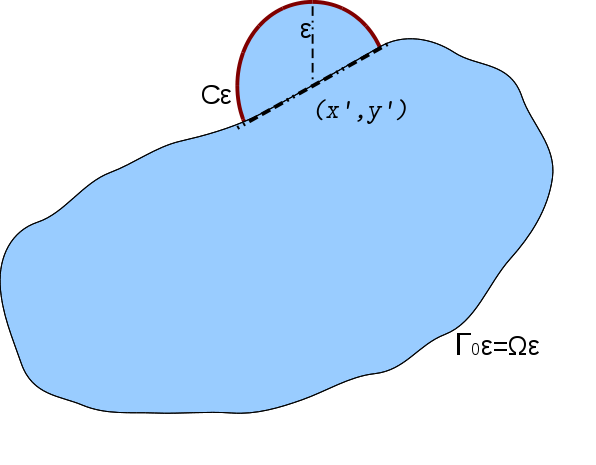
\includegraphics[height = 6cm]{lingkaran2.png}
\end{center}
 \caption{Domain to Avoid Singularity}\label{obstacleEpsilon}
\end{figure}

Let us approximate the integral on $\Gamma_0$ with an integral on $\Gamma_0^\varepsilon$
with $\varepsilon >0$.
From the Figure \ref{obstacleEpsilon}, as $\varepsilon\to0$, we expect $\integ{{\Gamma_0}^\varepsilon=\Omega_\varepsilon}{}{(\cdot)}\to\integ{\Gamma_0}{}{(\cdot)}$.
We know how to compute $\integ{{\Gamma_0}^\varepsilon=\Omega_\varepsilon}{}{(\cdot)}$, there are no singularities.

Let we calculate the Boundary Integral Formulation on the boundary. If $(x',y')\in \Gamma_0$, let we multiply equation
~\eqref{problem5} by $G_{x',y'} $ and integrate over $\Omega_\varepsilon$.
\begin{align}
\integ{\Omega_\varepsilon}{}{ \Delta \psi(x,y) G_{x',y'}(x,y)}=0\\
\integ{\partial\Omega_\varepsilon}{}{(G_{x',y'}\nabla \psi \cdot n) }-
\left\{\integ{\partial\Omega_\varepsilon}{}{\psi \nabla G_{x',y'}(x,y)\cdot n }-
\integ{\Omega_\varepsilon}{}{\psi (x,y)\Delta G_{x',y'}(x,y) }\right\}=0 \\
-\integ{\partial\Omega_\varepsilon}{}{G_{x',y'}u_0 n_x}-\integ{\partial\Omega_\varepsilon}{}{\psi \nabla G_{x',y'}\cdot n}+0=0\\
\integ{\partial\Omega_\varepsilon}{}{u_0 G_{x',y'}n_x+\psi \nabla G_{x',y'}\cdot n} =0 \label{BIboundary}
\end{align}

Let us examine $\integ{\partial\Omega_\varepsilon}{}{u_0 G_{x',y'}n_x+\psi \nabla G_{x',y'}\cdot n}$ as $\varepsilon\to0$
\begin{equation}
 \integ{\partial\Omega_\varepsilon}{}{u_0 G_{x',y'}n_x+\psi \nabla G_{x',y'}\cdot n}=
 \integ{C_\varepsilon}{}{u_0 G_{x',y'}n_x+\psi \nabla G_{x',y'}\cdot n}+
 \integ{\partial\Omega_\varepsilon\setminus C_\varepsilon}{}{u_0 G_{x',y'}n_x+\psi \nabla G_{x',y'}\cdot n}
\end{equation}
When $\varepsilon\to0$, if $\integ{\partial\Omega_\varepsilon\setminus C_\varepsilon}{}{u_0 G_{x',y'}n_x+\psi \nabla G_{x',y'}\cdot n}$ has a limit, then it is called The cauchy Principal Value. 
We denote it $\displaystyle\fpint{\partial\Omega}{}{u_0 G_{x',y'}n_x+\psi \nabla G_{x',y'}\cdot n}$.

let us examine $\integ{C_\varepsilon}{}{u_0 G_{x',y'}n_x+\psi \nabla G_{x',y'}\cdot n}$ as $\varepsilon\to0$.
\begin{align}
\integ{C_\varepsilon}{}{u_0 G_{x',y'}n_x+\psi \nabla G_{x',y'}\cdot n}
=& \integ{\theta^\ast}{\theta^\ast+\pi}{\left\{ \dfrac{1}{2\pi}\ln(\varepsilon) u_0 n_x+\psi \dfrac{1}{2\pi} \dfrac{1}{\varepsilon}\right\}\varepsilon \, d\theta }\\
=& \dfrac{1}{2\pi}\varepsilon\ln{\varepsilon}\integ{\theta^\ast}{\theta^\ast+\pi}{u_0 n_x \, d\theta}
+ \integ{\theta^\ast}{\theta^\ast+\pi}{\dfrac{1}{2\pi}\psi \, d\theta}\\
=&\integ{\theta^\ast}{\theta^\ast+\pi}{\dfrac{1}{2\pi}\psi \, d\theta}\\
=&\dfrac{1}{2\pi}\psi \integ{\theta^\ast}{\theta^\ast+\pi}{\, d\theta}\\
=& \dfrac{1}{2\pi}\psi(x',y') \label{residual}
\end{align}
Result from~\eqref{residual} is called a ``Residual Term''.

Now, we can compute~\eqref{BIboundary} when $\varepsilon\to0$ as follows:
\begin{align}
 \integ{\partial\Omega_\varepsilon}{}{u_0 G_{x',y'}n_x+\psi \nabla G_{x',y'}\cdot n}&=0\\
\fpint{\partial\Omega}{}{u_0 G_{x',y'}n_x+\psi \nabla G_{x',y'}\cdot n}+\dfrac{1}{2\pi}\psi(x',y')&=0\\
\dfrac{1}{2\pi}\psi(x',y')=-\fpint{\partial\Omega}{}{u_0 G_{x',y'}n_x+\psi \nabla G_{x',y'}\cdot n}\label{BIboundary1}
\end{align}
Next, we can calculate all these terms with numerical method.

\section{Numerical Methods}
\subsection{Solving Boundary Integral Formulation on an Obstacle}

We want to solve numerically Boundary Integral Formulation on the ostacle as we get in equation~\eqref{BIboundary1}. 
First, we consider that on the boundary of obstacle, we have N partitions. In each partitions we have
$\psi_i=\psi(x_i,y_i)$ and 
 \[ e_i(x,y) = \left\{
  \begin{array}{l l}
    1 & \quad \text{if $(x,y)\in S_i$ }\\
    0 & \quad \text{otherwise}
  \end{array} =\chi_{S_i}\right.\]
We obtain the value of $\psi$ as
\begin{equation}
 \psi(x,y)=\sum\limits_{i=1}^N \psi_i e_i(x,y)
\end{equation}

picture here...

For $i$ from 1 to $n$ we can write~\eqref{BIboundary1} as 
\begin{align}
 \underbrace{\dfrac{1}{2\pi}\psi(x_i,y_i)}_\text{1} + 
   \underbrace{\fpint{\partial\Omega}{}{\psi \nabla G_{x_i,y_i}\cdot n}}_\text{2}=\underbrace{-\fpint{\partial\Omega}{}{G_{x_i,y_i}u_0n_x}}_\text{3} \label{BIboundary2}
\end{align}
Let we see each items:
\begin{enumerate}
 \item $ \dfrac{1}{2\pi}\psi(x_i,y_i) = \dfrac{1}{2\pi}\psi_i$  

 \item $\displaystyle\fpint{\partial\Omega}{}{\psi \nabla G_{x_i,y_i}\cdot n}=\displaystyle\fpint{\partial\Omega}{}{\left\{\sum\limits_{j=1}^N \psi_j e_j\right\} \nabla G_{x_i,y_i}\cdot n}$
 \begin{align}
\fpint{\partial\Omega}{}{\psi \nabla G_{x_i,y_i}\cdot n}&=\fpint{\partial\Omega}{}{\left\{\sum\limits_{j=1}^N \psi_j e_j\right\} \nabla G_{x_i,y_i}\cdot n}\\
&=\fpint{\partial\Omega}{}{\left\{\sum\limits_{j=1}^N \psi_j \varepsilon_j\nabla G_{x_i,y_i}\cdot n\right\} }\\
&= \sum\limits_{j=1}^N \left\{ \displaystyle\fpint{\partial\Omega}{}{\psi_je_j\nabla G_{x_i,y_i}\cdot n } \right\}\\
&=\sum\limits_{j=1}^N \psi_j \left\{ \displaystyle\fpint{\partial\Omega}{}{\nabla G_{x_i,y_i}\cdot n e_j} \right\}\\
&=\sum\limits_{j=1}^N\psi_j \left\{ \fpint{S_j}{}{\nabla G_{x_i,y_i}\cdot n} \right\}\\
&=\sum\limits_{j=1}^N \psi_j m_{ij}=(M\psi)_i
\end{align}
with $
      M=(m_{ij})_{\substack{i=1 \cdots N \\j=1 \cdots N}}
     $
and
$
\psi=(\psi_j)_{j=1,\cdots,N}. 
$

\item $-\displaystyle \fpint{\partial\Omega}{}{G_{x_i,y_i}u_0n_x}$

Since the domain is divided in line, we have $n=\left( \begin{array}{c}
      n_x \\
      n_y
    \end{array}\right)$
and $n_x=\sum\limits_{i=1}^N n_{x_i}e_i$,  $n_y=\sum\limits_{i=1}^N n_{y_i}e_i$.

\begin{align}
-\fpint{\partial\Omega}{}{G_{x_i,y_i} u_0 n_x} &= -u_0 \fpint{\partial\Omega}{}{G_{x_i,y_i} n_x} =
-u_0 \fpint{\partial\Omega}{}{G_{x_i,y_i} \sum\limits_{j=1}^N n_{x_j}e_j}\\
&= -u_0 \fpint{\partial\Omega}{}{\sum\limits_{j=1}^N n_{x_j}e_j G_{x_i,y_i}}\\
&= -u_0\sum\limits_{j=1}^N \fpint{\partial\Omega}{}{n_{x_j}e_j G_{x_i,y_i}}\\
&= -u_0\sum\limits_{j=1}^N n_{x_j} \fpint{\partial\Omega}{}{G_{x_i,y_i}e_j}\\
&=-u_0 \sum\limits_{j=1}^N n_{x_j} \integ{S_j}{}{G_{x_i,y_i}}\\
&=-u_0 (P N_x)_i
\end{align}
\end{enumerate}

We will compute matrices $P=(p_{i,j})=\integ{S_j}{}{G_{x_i,y_i}}$ and $M=(m_{i,j})=\displaystyle \fpint{S_j}{}{\nabla G_{x_i,y_i}\cdot n}$ which the calculating process divides in two cases.
\begin{enumerate}
 \item $i\neq j$

Let we see the point $(x_i,y_i)$ towards the other points in partition. Since $\nabla G_{x_i,y_i}$ and $G_{x_i,y_i}$ are radial functions, we can turn the axis in such a way more convenient to examine. 
In picture.... we change the coordinate $xu$ with $\eta \nu$

In $\eta \nu$ coordinate, we can write Green function $G$ as
\begin{equation}
  G_{x_i,y_i}(\eta,\nu)=\frac{1}{2\pi} \ln\left(\sqrt{\eta^2 + \nu^2}\right)
\end{equation}
we can also write $\eta$ and $\nu$ in radial coordinates as follows:
\begin{align}
 \eta=r \cos\theta=H\\
\nu=r \sin\theta\\
\frac{\nu}{\eta}=\tan \theta \Leftrightarrow \nu=\eta \tan \theta
\end{align}
along the integration line, $\eta=H$. 
\begin{equation}
  \nu=H\tan\theta\Leftrightarrow d\nu=H \frac{1}{\cos^2\theta}= H \sec^2\theta d\theta
\end{equation}
With using these values, we can get
\begin{align}
 p_{ij}&=\fpint{S_j}{}{G_{x_i,y_i}}=\fpint{\nu_{j-\frac{1}{2}}}{\nu_{j+\frac{1}{2}}}{G_{x_i,y_i}(H, \nu) \, d\theta}\\
&=\fpint{\theta_{j-\frac{1}{2}}}{\theta_{j+\frac{1}{2}}}{\frac{1}{2\pi} 
\left( \ln(H\sec \theta) H \sec^2\theta \right)  \, d\theta}\\
&=\frac{H}{2\pi} \fpint{\theta_{j-\frac{1}{2}}}{\theta_{j+\frac{1}{2}}}{\ln(H\sec\theta) H \sec^2\theta \mathrm{d}\theta}\\
&=\frac{H}{2\pi}\left [ \tan \theta \ln (H\sec\theta)+\theta-\tan\theta \right ]_{\theta_{j-\frac{1}{2}}}^{\theta_{j+\frac{1}{2}}}
\end{align}
\begin{align}
 m_{ij}&=\fpint{S_j}{}{\nabla G{x_i,y_i}(H,\nu)\cdot n}\\
 &=\fpint{S_j}{}{\frac{1}{2\pi} \left( \begin{array}{c}
      \frac{2\eta}{2 \sqrt{\eta^2 + \nu^2} }\frac{1}{\sqrt{\eta^2 + \nu^2}} \\
      \frac{2\nu}{2 \sqrt{\eta^2 + \nu^2}} \frac{1}{\sqrt{\eta^2 + \nu^2}}
    \end {array} \right) \cdot n }=
        \fpint{S_j}{}{ \frac{1}{2\pi} \frac{1}{\eta^2 + \nu^2} \left(\begin{array}{c}
      \nu \\
      \eta
    \end{array}\right) \cdot n \, d\nu}\\
&=\fpint{\theta_{j-\frac{1}{2}}}{\theta_{j+\frac{1}{2}}}{\frac{1}{2\pi} \frac{1}{r^2} \left(\begin{array}{c}
      r \cos\theta \\
      r \sin \theta
    \end{array}\right)\cdot\left(\begin{array}{c}
      -1 \\
      0
    \end{array}\right)H \sec^2\theta \, d\theta}\\
&=\fpint{\theta_{j-\frac{1}{2}}}{\theta_{j+\frac{1}{2}}}{\frac{-\cos\theta}{2\pi r}H \sec^2\theta \, d\theta}\\
&=\fpint{\theta_{j-\frac{1}{2}}}{\theta_{j+\frac{1}{2}}}{\frac{1}{2\pi H\sec^2\theta}H \sec^2\theta \, d\theta}\\
&=- \frac{1}{2\pi} \fpint{\theta_{j-\frac{1}{2}}}{\theta_{j+\frac{1}{2}}}{\, d\theta}\\
&=-\frac{1}{2\pi}(\theta_{j+\frac{1}{2}}-\theta_{j-\frac{1}{2}})
\end{align}

 \item $i=j$
 
picture here.....

\begin{align}
 P_{ij}=&\fpint{S_i}{}{G_{x_i,y_i}}\\
 =&\lim_{\varepsilon \to 0} \integ{\nu_{i-\frac{1}{2}}}{-\varepsilon}{G_{x_i,y_i}(0,\nu) \, d\nu} + \integ{\varepsilon}{\nu_{i+\frac{1}{2}}}{G_{x_i,y_i}(0,\nu) \, d\nu}\\
 =&\lim_{\varepsilon \to 0} \integ{\nu_{i-\frac{1}{2}}}{-\varepsilon}{\frac{1}{2\pi}\ln \left( \sqrt{0 + \nu^2}\right) \, d\nu}+
 \integ{\varepsilon}{\nu_{i+\frac{1}{2}}}{\frac{1}{2\pi}\ln \left( \sqrt{0 + \nu^2}\right) \, d\nu}\\ 
   =&\lim_{\varepsilon \to 0} \integ{-\frac{l_i}{2}}{-\varepsilon}{\frac{1}{2\pi}\ln\left( \lvert \nu \rvert \right) \, d\nu}+ 
 \integ{\varepsilon}{\frac{l_i}{2}}{\frac{1}{2\pi} \ln\left( \lvert \nu \rvert \right) \, d\nu}\\
 =&\frac{2}{2\pi} \lim_{\varepsilon \to 0} \integ{\varepsilon}{\frac{l_i}{2}}{\frac{1}{2\pi}\ln \left( \nu \right) \, d\nu}\\
 =&\frac{1}{\pi} \lim_{\varepsilon \to 0} \left(\nu \ln\nu-\nu \right)_\varepsilon^{\frac{l_i}{2}}\\
 =&\frac{1}{\pi} \lim_{\varepsilon \to 0} \left\{ \left( \frac{l_i}{2}\ln \left( \frac{l_i}{2} \right)-\frac{l_i}{2} \right)- \left( \varepsilon \ln\varepsilon- \varepsilon \right) \right\}\\
=& \frac{1}{\pi} \left( \frac{l_i}{2}\ln \left( \frac{l_i}{2} \right)-\frac{l_i}{2} \right)
 \end{align}
 
 As long as $G$ is a radial function, $\nabla G$ is also radial (radial vector). We obtain 
\begin{align}
 m_{ij}&=\fpint{S_j}{}{\nabla G{x_i,y_i}\cdot n}\\
 &=\lim_{\varepsilon \to 0} \integ{-\frac{l_i}{2}}{-\varepsilon}{\nabla G{x_i,y_i}\cdot n (0,\nu)}+ \integ{\varepsilon}{\nu_{i+\frac{1}{2}}}{\nabla G{x_i,y_i}\cdot n (0,\nu)}\\
 &=\lim_{\varepsilon \to 0} \integ{-\frac{l_i}{2}}{-\varepsilon}{\frac{1}{2\pi} \frac{1}{\eta^2+\nu^2} \left(\begin{array}{c}
      \nu \\
      \eta
    \end{array}\right) \left(\begin{array}{c}
      -1 \\
      0
    \end{array}\right) (0,\nu)}+\integ{\varepsilon}{\nu_{i+\frac{1}{2}}}{\frac{1}{2\pi} \frac{1}{\eta^2+\nu^2} \left(\begin{array}{c}
      \nu \\
      \eta
    \end{array}\right) \left(\begin{array}{c}
      -1 \\
      0
    \end{array}\right) (0,\nu)}\\
&=0
\end{align}
 
\end{enumerate}

From the calculation above, we can write~\eqref{BIboundary2} as following equation  system:
\begin{equation}\label{SPL}
 \left( \frac{1}{2} I+M \right) \psi= -u_0 P N_x 
\end{equation}
with 
\[  m_{ij}= \left\{
  \begin{array}{l l}
    0 & \quad \text{if $i=j$ }\\
    -\frac{1}{2\pi}(\theta_{j+\frac{1}{2}}-\theta_{j-\frac{1}{2}}) & \quad \text{otherwise}
  \end{array} \right.\]
  and
  \[  p_{ij}= \left\{
  \begin{array}{l l}
     \frac{1}{\pi} \left( \frac{l_i}{2}\ln \left( \frac{l_i}{2} \right)-\frac{l_i}{2} \right) & \quad \text{if $i=j$ }\\
    \frac{H}{2\pi}\left [ \tan \theta \ln (H\sec\theta)+\theta-\tan\theta \right ]_{\theta_{j-\frac{1}{2}}}^{\theta_{j+\frac{1}{2}}} & \quad \text{otherwise}
  \end{array} \right.\]

\subsection{Solving Boundary Integral Formulation in Domain}

We have to solve boundary integral formulation in domain $(x',y')\in \Omega$ as in equation~\eqref{BIform}. 
\begin{equation}
 \psi_{x',y'}(x,y)=-\integ{\Gamma_0}{}{(-u_0 n_x)G_{x',y'}(x,y)} + \integ{\Gamma_0}{}{\psi\nabla G_{x',y'}(x,y)\cdot \vec{n}} \label{BIform1}
\end{equation}
If we call $-u_0 n_x$ and $\psi$ respectively with Neum and Diri, we can write \ref{BIform1} as
\begin{equation}
 \psi_{x',y'}(x,y)=-\integ{\Gamma_0}{}{\text{Neum}G_{x',y'}(x,y)} + \integ{\Gamma_0}{}{\text{Diri}\nabla G_{x',y'}(x,y)\cdot \vec{n}}
\end{equation}

For solving Boundary Integral Formulation inside the domain, in order to get the potential flow, we wish to obtain $u=\nabla\psi$.
\begin{equation}
 \nabla\psi=\left(\begin{array}{c}
      \partial_{x'}\psi \\
      \partial_{y'}\psi
    \end{array}\right)
\end{equation}
 We have to compute $\partial_{x'}\psi$.
\begin{align}
 \partial_{x'}\psi(x',y')&=\partial_{x'}\left(-\integ{\Gamma_0}{}{\text{Neum}G_{x',y'}(x,y)} + \integ{\Gamma_0}{}{\text{Diri}\nabla G_{x',y'}(x,y)\cdot \vec{n}} \right)\\
&=  \underbrace{-\integ{\Gamma_0}{}{\text{Neum} \left(\partial_{x'}G_{x',y'}(x,y)\right)}}_\text{1}  +  
\underbrace{\integ{\Gamma_0}{}{\text{Diri}\left(\partial_{x'}\nabla G_{x',y'}(x,y)\cdot \vec{n}\right)}}_\text{2} 
\end{align}

\begin{enumerate}
 \item We have to find the value of $-\integ{\Gamma_0}{}{\partial_{x'} G_{x',y'} \text{Neum}}$

We use Green function as in equation \ref{GreenFunction}. We obtain its derivative to $x'$ as follow:
\begin{equation}
 \partial_{x'} G_{x',y'}(x,y)=-\frac{1}{2}\frac{x-x'}{(x-x')^2+(y-y')^2}
\end{equation}
We can see point $(x',y')$ in coordinate $(x,y=u)$ in figure \ref{PointsDomain}. we also can turn the axis and ordinat in such a convenient way as we see in figure \ref{turnAxis}. 
\begin{figure}[!htbp]
\begin{center}
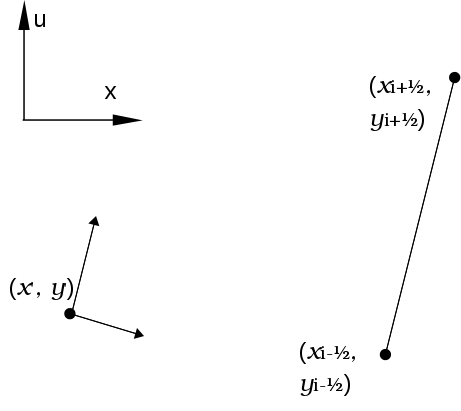
\includegraphics[height = 6cm]{positionOfPoints.png}
\end{center}
 \caption{Points in Domain}\label{PointsDomain}
\end{figure}

\begin{figure}[!htbp]
\begin{center}
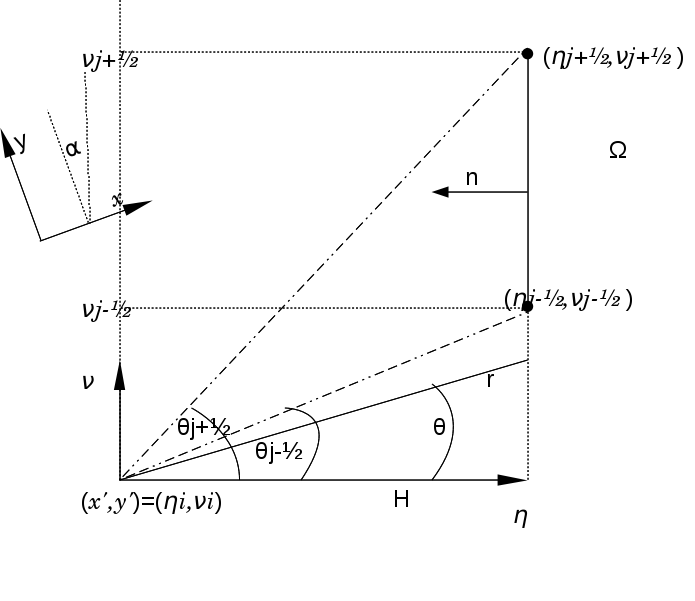
\includegraphics[height = 10cm]{changeAxis.png}
\end{center}
 \caption{Change the axis and ordinat}\label{turnAxis}
\end{figure}
in $\eta\nu$ coordinate, along the integration line, we get:
\begin{align}
 x-x'&=\eta=r \cos \theta=H \quad\text{,} r=H\sec\theta\\
y-y'&=\nu= r\sin \theta\\
\frac{\eta}{\nu}= \tan\theta\\
\nu=\eta \tan \theta=H\tan \theta\\
\d \nu=H \sec^2\theta \d \theta
\end{align}
Let us compute the integral
\begin{align}
 -\integ{\Gamma_0}{}{\partial_{x'} G_{x',y'} \text{Neum}}&=-\sum\limits_{i=1}^N  \integ{S_i}{}{\partial_{x'} G_{x',y'} \text{Neum} \, dS}\\
&=-\sum\limits_{i=1}^N \text{Neum} \integ{\nu_{i-\frac{1}{2}}}{\nu_{i+\frac{1}{2}}}{\partial_{x'} G_{x',y'} (H,\nu) \, d\nu}\\
&=-\sum\limits_{i=1}^N \frac{-\text{Neum}}{2\pi} \integ{\theta_{i-\frac{1}{2}}}{\theta_{i+\frac{1}{2}}}{\frac{H}{\left( H\sec\theta\right)^2 }H \sec^2\theta \, d\theta}\\
&=-\sum\limits_{i=1}^N \frac{-\text{Neum}}{2\pi} \integ{\theta_{i-\frac{1}{2}}}{\theta_{i+\frac{1}{2}}}{\, d\theta}\\
&=\sum\limits_{i=1}^N \frac{\text{Neum}}{2\pi} \left( \theta_{i+\frac{1}{2}}- \theta_{i-\frac{1}{2}} \right)
\end{align}

\item We have to compute $\integ{\Gamma_0}{}{\partial_{x'}\nabla G_{x',y'} \cdot n \text{diri}}$
\end{enumerate}



\end{document}
